\chapter{Server design and development}
\label{ch:server}

In this chapter, the general model behind the server will be elaborated. The formal documentation with descriptions of the server classes and their methods can be found on page~\pageref{app:documentation}, which also includes an UML class diagram \cite{uml}. An HTML version is also available on \url{mvdenk.com/thesis/doc/}. The description of the model is divided in generic data entries --- entailing the supplanted data by the developer such as the concept map or test items --- and the user attributes, objects and methods --- entailing user specific data such as birthdate or how often a user responded correctly or incorrectly to a certain instance. Only the conceptually relevant methods will be described below, since this keeps the thesis more accessible for readers not familiar with programming paradigms, and these methods are already described within the documentation. For example, the to\_dict() method is prevalent in a large amount of classes, but merely serves the purpose of converting the class into an object that can be sent over the network connection to and rendered within the client and therefore is not conceptually relevant and is not elaborated. The two classes left out of the description are the Controller class, which parses client messages, operates the server and translates the server output to a new network message, and the LogEntry, which represents a single incoming or outgoing network message. These classes are also not conceptually relevant, and their functionality can already be derived from the previously described UML Activity Diagrams in figure~\ref{fig:loginactivity} on page~\pageref{fig:loginactivity} and figure~\ref{fig:learningactivitygen} on page~\pageref{fig:learningactivitygen}.

\section{Generic data entries}

There are four classes of generic data: the concept map (containing nodes and edges), the flashcards, the test items and the questionnaire items. The concept map and flashcard model is illustrated in figure~\ref{fig:classdiagram_concept_map}.

\begin{figure}
    \centering
    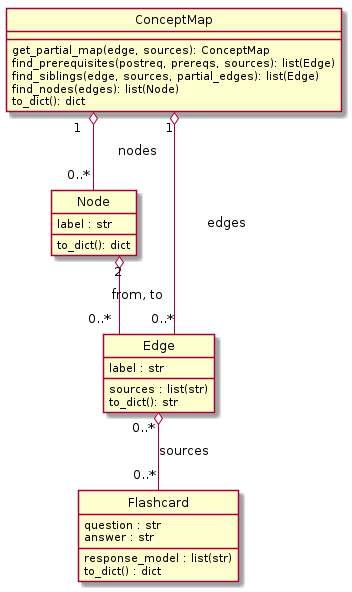
\includegraphics[height=0.4\textheight]{img/classdiagram_concept_map.png}
    \caption{A UML class diagram illustrating the ConceptMap, Node, Edge, and Flashcard classes}
    \label{fig:classdiagram_concept_map}
\end{figure}

\subsection{Concept map}

The ConceptMap class is mainly a container class consisting of nodes and edges, and certain useful methods for performing standard queries on the concept map. As described in the general definition of the concept map by \citeA{canas}, a Node object represents a concept, and an Edge object represents a relation between two concepts. The Node and Edge were originally intended to be embedded within the ConceptMap class, however this makes them impossible to refer to by other classes in MongoEngine (used for interacting with the MongoDB database). Furthermore, it could theoretically be possible for certain Nodes to exist in different concept maps. Therefore, they are implemented as separate classes in this server model. The example concept map in figure~\ref{fig:examplemap} is used to demonstrate the different functions in of the class.

\begin{figure}
    \centering
    \begin{subfigure}{0.4\textwidth}
        \centering
        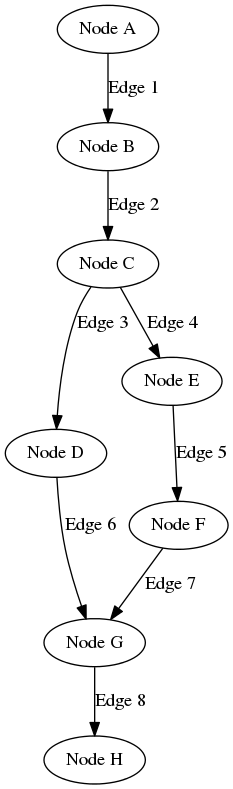
\includegraphics[height=.6\textheight]{img/examplemap.png}
        \caption{An abstract example of a concept map}
        \label{fig:examplemap}
    \end{subfigure}
    \qquad
    \begin{subfigure}{0.4\textwidth}
        \centering
        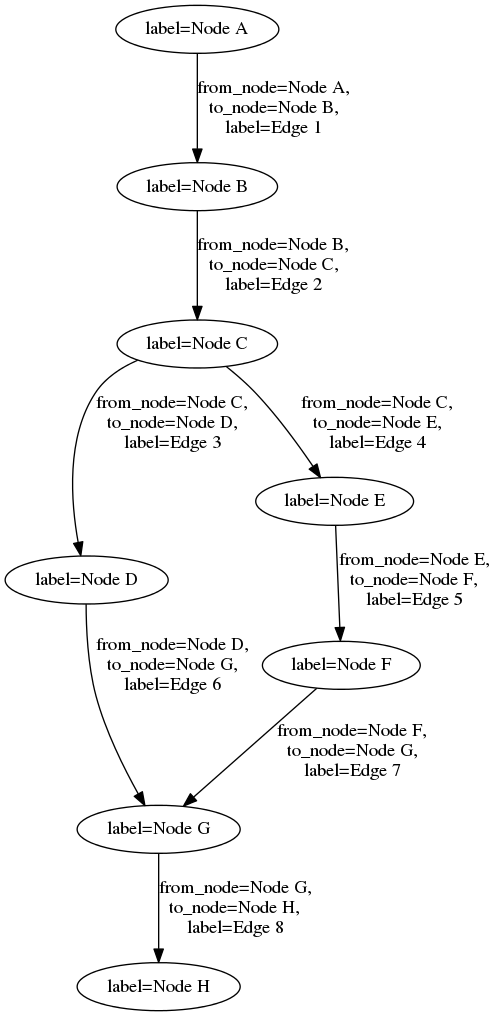
\includegraphics[height=.6\textheight]{img/examplemap_objects.png}
        \caption{The different attributes demonstrated within the example map from figure~\protect\ref{fig:examplemap}}
        \label{fig:examplemap_objects}
    \end{subfigure}
    \caption{An example illustrating the ConceptMap class}
    \label{fig:examplemaps}
\end{figure}

\paragraph{Nodes} The concepts represented by the nodes are not only an abstract ideas (such as Renaissance Literature), but also more concrete concepts such as a time period (e.g. the Golden Age), a person (e.g. P.C. Hooft) or objects or inventions (e.g. the printing press). Nodes are simple classes only containing a label describing what it should represent and a unique identifyer string.

\paragraph{Edges} An Edge also contains a label describing the specific relation between two concepts and an id, but also contains the references to the id's of the nodes it refers to, one being the `from' node and the other the `to' node, and a list of sources (usually only containing one source), which are the sections of the instructional material the edge is derived from. The model does not make any destinction between a hierarchical and cross-link, since they are the same from a graph rendering perspective. However, this destinction might still be considered for more sophisticated hierarchical rendering or searching algorithms. The Edge class is chosen as the equivalent to the Flashcard in the Flashmap system rather than the Node, since a relation between concepts is more specific when teaching about concepts. Furthermore, within an Edge object there is already a clear question (the from\_node) and answer (the to\_node).

Figure~\ref{fig:examplemap_objects} demonstrates how the different classes and attributes represent the concept map from figure~\ref{fig:examplemap}.

\paragraph{Methods} The most important method of the ConceptMap class is the get\_partial\_map() function, which will provide a new ConceptMap object containing all the parent nodes and edges which directly or indirectly link to a given Node (the parent nodes and edges), plus the nodes and edges linked to by the direct parent nodes (the sibling nodes and edges). This concept map can then be displayed to the user when showing a specific flashmap instance for review. The reason why the parent nodes are returned rather than the child nodes is that in the instructional material the concepts are introduced top-down rather than bottom up, so building up the concept map from parent to child alligns better with the order in which the students read about the concepts. Additionally, the sibling nodes are also returned so that they can be prompted at the same time, and that the user has more context for deciding which concept should be filled in the missing node. Figure~\ref{fig:examplemap_partial_d} and figure~\ref{fig:examplemap_partial_g} demonstrate the get\_partial\_map() function with Node D and Node G from the example map in figure~\ref{fig:examplemap}.

\begin{figure}
    \centering
    \begin{subfigure}{0.4\textwidth}
        \centering
        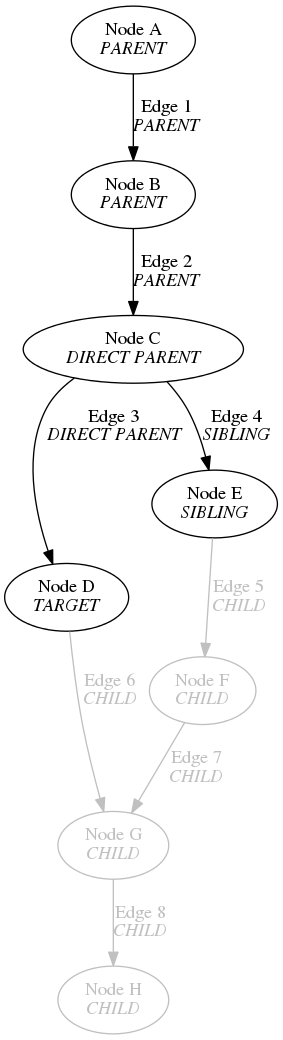
\includegraphics[height=.6\textheight]{img/examplemap_partial_d.png}
        \caption{The result of get\_partial\_map() function with Node D from the example map from figure~\protect\ref{fig:examplemap}}
        \label{fig:examplemap_partial_d}
    \end{subfigure}
    \qquad
    \begin{subfigure}{0.4\textwidth}
        \centering
        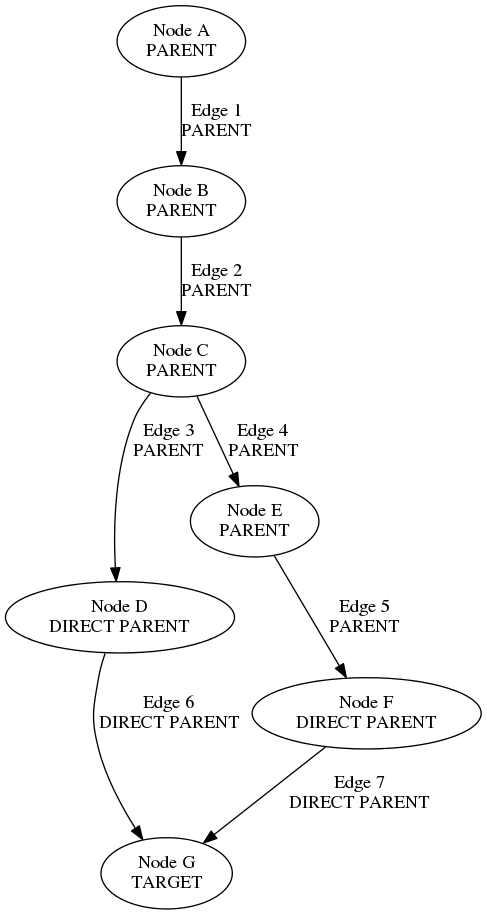
\includegraphics[height=.6\textheight]{img/examplemap_partial_g.png}
        \caption{The result of get\_partial\_map() function with Node G from the example map from figure~\protect\ref{fig:examplemap}}
        \label{fig:examplemap_partial_g}
    \end{subfigure}
    \caption{Example for using the get\_partial\_map() function of the ConceptMap class}
    \label{fig:examplemap_partial}
\end{figure}

\subsection{Flashcards}

A Flashcard class represents a traditional flashcard by simply having a question and answer entry. It addtitionally has an response model entry in order to also function as a test item. In most cases, this is a list only containing the answer entry, however in some cases the answer entry is split into multiple response entries. Finally, since each flashmap is based on the concept map, each Flashcard object also contains a list with Edges the card is derived from. This has the advantage of being able to compare the flashcards with the concept map, but also indirectly relates the flashcards to the sections within the instructional material.

\subsection{Test items}

A TestItem object represents an item on the pre- or posttest. It is very similar to a Flashcard object, with the exception that it directly links to the text sources, and does not contain an answer field since this is never displayed to the user.

\subsection{Questionnaire items}

The QuestionnaireItem class represents items from the Technology Acceptance Model questionnaire \cite{tamq}, and contains a usefulness entry categorising the item as either a Perceived Usefulness item or as a Perceived Ease of Use item, and a positive and a negative phrasing entry. Both phrasings are included instead of only the standard positive phrasing, so that one of these phrasings can be selected when presenting the item to the user, avoiding only one type of phrasing causing a bias within the user towards that specific phrasing.

\section{User attributes, objects and methods}

The main user attributes are mainly based on the aforementioned generic data entries, namely the FlashcardInstance or FlashmapInstance objects --- storing the learning progression of certain Flashcards or Edges from the ConceptMap ---, the Test objects --- representing a pre- or posttest and containing the responses to sets of TestItems ---, and the Questionnaire object --- containing the responses to the QuestionnaireItems. Next to these objects, the user also has certain descriptive attributes, and objects related to logged in sessions. The User class and its attributes and embedded classes are illustrated in figure~\ref{fig:classdiagram_user}.

\begin{figure}
    \centering
    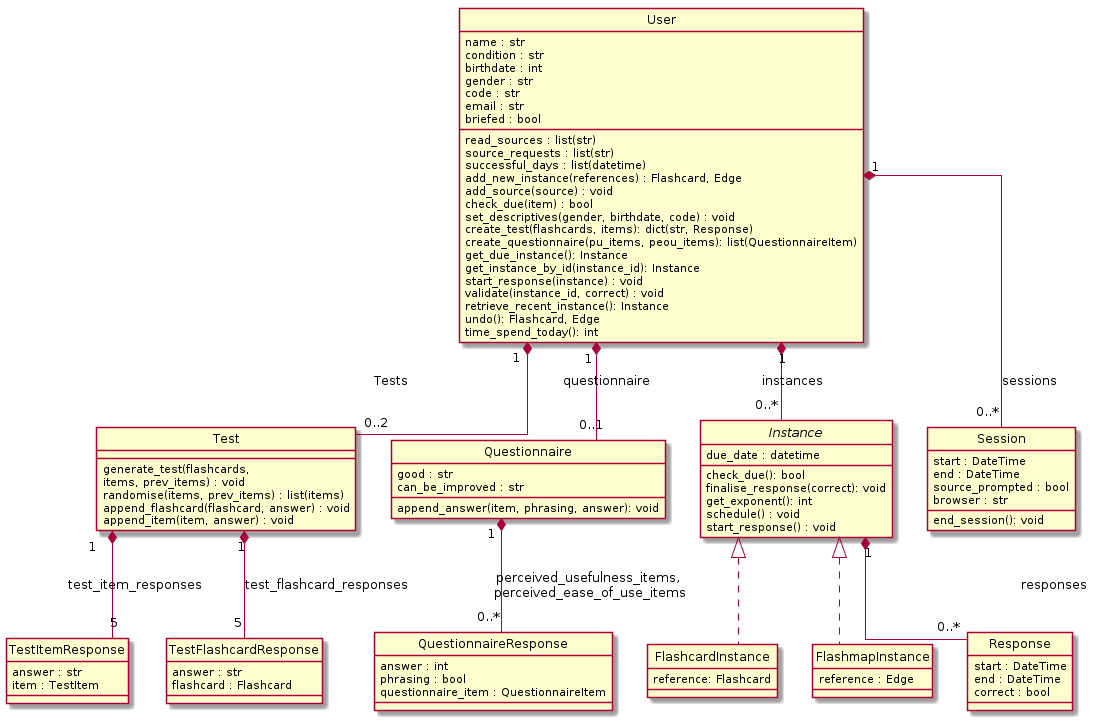
\includegraphics[width=\textwidth]{img/classdiagram_user.png}
    \caption{A UML class diagram illustrating the User class and its embedded classes. For readability, the TestItem, QuestionnaireItem, Flashcard and Edge classes are referred to inline within the attributes instead of as separate classes with aggregation links.}
    \label{fig:classdiagram_user}
\end{figure}

\subsection{Descriptive attributes}

The descriptive attributes are either used for the program to function, or for generating descriptive statistics as controll variables in the results section. They contain the username, the condition, the gender and birthdate of the user, the code he received on his informed consent form, an email address, and a debriefed field.

\paragraph{Username} First and foremost, every user has a unique username which can be used to log in to the application. This name is chosen by the user himself, so he can decide to use his proper name or use an alias to remain anonymous. Even so, within the released data this field is removed in order to safeguard the identities of the user.

\paragraph{Condition} This field determines whether the user is partaking in the "FLASHCARD" group (the control group) or the "FLASHMAP" group (the experimental group). This field is set when the user registers a new account by the formula $len(users) \bmod 2$, which entails that every new user is assigned to the opposite group relative to the user before. This is in order to ensure that the initial users are equally divided over both groups.

\paragraph{Gender} The gender field of the user is included in order to check after the experiment whether the distribution of genders is equal within both experimental conditions. This variable is prompted before the pretest.

\paragraph{Birthdate} The birthdate field of the user is included in order to check after the experiment whether the age distributions of both experimental conditions are the same. This variable is prompted before the pretest.

\paragraph{Code} Before the start of the experiment, every student participating had to sign an informed consent form together with a parent or caretaker in accordance with the Ethics Committee at the University of Twente. To ensure that every user in the system corresponded with students who handed in a double signed form without the user having to enter his own name into the system, every form contained a code which was prompted towards the user before the pretest.

\paragraph{Email} At the end of the questionnaire, the user was prompted whether he wanted to participate in an interview. If this was the case, he could fill in his email address here in order to be contacted at a later date. This variable is also ommitted in the published data.

\paragraph{Debriefed} This field is a simple boolean value indicating whether the user has been debriefed. It initiated with a False value, and was set to True when the server received a "DEBRIEFING-RESPONSE" message from the client (see figure~\ref{fig:loginactivity} on page~\pageref{fig:loginactivity}).

\subsection{Sessions}

A Session object represents the time between the user logs in and out. This is represented by a \emph{start} and \emph{end} value, indicating the time interval and the moment that the user was active. Additionally, the Session object has a variable \emph{source\_prompted}, indicating whether the user was prompted to read a section within the instructional material. The object finally contains a string \emph{browser}, which is the string retrieved from navigator.platform in the client window.

\subsection{Instances}

The instances class is the most relevant class for the functioning of the flashcard system, containing a record of responses and the scheduling function. The name instance is used in order to distinguish between an abstract Flashcard or Edge, which is the same for each user, and the specific instance of this idea within the memory of a user. An Instance object can be either a FlashcardInstance or a FlashmapInstance, depending of the experimental condition of the user.

\paragraph{Attributes} Each Instance object has a \emph{due\_date} and \emph{reference} attribute. The \emph{due\_date} attribute indicates when this instance is due for review by the user, and initiates at the current date and time. This date is set by the scheduling function, which is elaborated below. The reference attribute contains either a Flashcard or an Edge object. As already indicated in the previous chapter, each time the user has no more due instances a new instance is created referring to a new item. The \emph{reference} field refers to either a Flashcard or an Edge, depending on the specific subclass of Instance.

\paragraph{Responses} The Response class represents each individual time the user reviews an instance, containing a \emph{start} field for when the Flashcard or Edge was prompted, an \emph{end} field for when the server received the response from the user, and a \emph{correct} field for whether the user was able to think of the correct answer or to\_node when being prompted.

\paragraph{Schedule} The scheduling algorithm uses two different methods from Instances, namely get\_exponent() and schedule(), and is illustrated in figure~\ref{fig:learningserver}. In the~\nameref{ch:frameworks} chapter on page~\pageref{ch:frameworks}, it is described that to calculate the interval until the next review, one needs the number of correct responses since the last incorrect response. This is done by the get\_exponent() function, which loops through the responses in descending order of \emph{end} date, increasing a counter (exp, initiated with value 1), until a response with a False \emph{correct} value is found. The schedule() function then takes $5^(exp)$ seconds as the interval until the next review of the instance. Examples:
%
\begin{itemize}
        \item When there are no responses, the interval is $5^1=5$ seconds;
        \item When there are three correct responses, the interval is $5^3=125$ seconds;
        \item When there are two correct responses, followed by one incorrect response and then 4 correct responses, the interval is $5^4=625$ seconds.
\end{itemize}
%
This interval is then added together with the \emph{end} value of the last response and sets this as the new \emph{due\_date} value.

\begin{figure}
\centering
    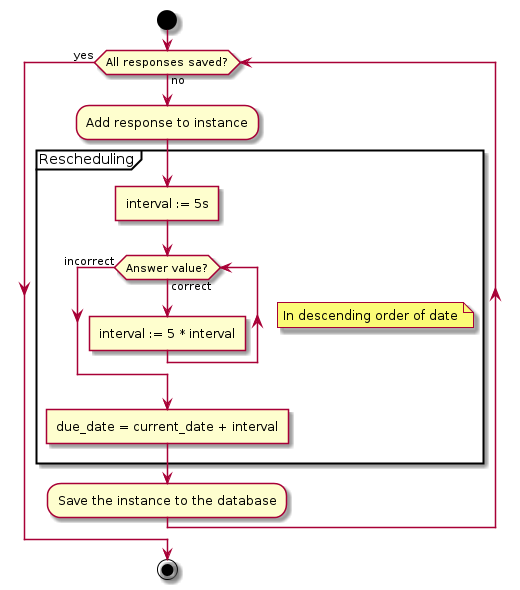
\includegraphics[height=.5\textheight]{img/learningserver.png}
\caption{An UML activity diagram showing the scheduling and saving of a list of responses within instances}
\label{fig:learningserver}
\end{figure}

\subsection{Tests}

\subsection{Questionnaire}
